% Appendix Template

\chapter{OVITO} % Main appendix title

\label{AB} % Change X to a consecutive letter; for referencing this appendix elsewhere, use \ref{AppendixX}

\lhead{Anexo B. \emph{OVITO}} % Change X to a consecutive letter; this is for the header on each page - perhaps a shortened title

Ciertas imágenes (por ejemplo las figuras \ref{C4:fg:fcc_tension_bmg_10K} y \ref{C5:fg:ss_comp}) fueron realizadas utilizando el software Ovito \citep{stukowski10}. En el presente apéndice explicaremos cómo obtener dichas imágenes y daremos recomendaciones para mejorar el uso del software. Como condición previa es necesario haber instalado y ejecutado LAMMPS (Apéndice \ref{AA}), ya que Ovito trabaja, entre otras cosas, con los archivos de salida de éste.

\section{Instalación}
\label{AB_1}

Ovito es una software libre para la visualización. Es posible descargarlo para diversas plataformas en el \href{http://www.ovito.org/index.php/download}{sitio web}. Siendo usuarios linux, explicaremos únicamente para un sistema operativo tipo linux.

La instalación de Ovito es considerablemente más sencilla que la de LAMMPS. Basta con descomprimir el archivo descargado y ejecutar \textit{bin/ovito}. Sin embargo puede ser útil copiar las carpetas \textit{bin}, \textit{lib} y \textit{share} a \textit{usr/local/} para poder acceder a los ejecutables a través de línea de comando sin tener que acceder a la carpeta descargada.

En ocasiones puede ser útil descargar el código fuente, puesto que podemos contar con actualizaciones del código de Ovito para las cuales tendríamos que esperar hasta que se presente la siguiente versión estable. Para ello, accedemos al \href{http://sourceforge.net/p/ovito/git/ci/master/tree/}{repositorio Git en Sourceforge.net}, descargamos el archivo y seguimos las \href{http://www.ovito.org/manual/development.build_linux.html}{instrucciones}.

\begin{lstlisting}
sudo apt-get install build-essential git cmake-curses-gui qt5-default libcgal-dev libboost-dev \
		     libqt5scintilla2-dev libavcodec-dev libavdevice-dev libavfilter-dev \
		     libavformat-dev libavresample-dev libavutil-dev libswscale-dev libnetcdf-dev \
		     libhdf5-dev libhdf5-serial-dev libbotan1.10-dev libmuparser-dev python3-dev \
		     libboost-python-dev python3-sphinx python3-numpy xsltproc docbook-xml \
		     docbook-xsl docbook-xsl-doc-html doxygen
                     
cd ovito
mkdir build
cd build
cmake -DOVITO_BUILD_DOCUMENTATION=ON \
      -DCMAKE_BUILD_TYPE=Release \
      -DPYTHON_INCLUDE_DIR=/usr/include/python3.4m \
      -DPYTHON_LIBRARY=/usr/lib/x86_64-linux-gnu/libpython3.4m.so \
      -DBoost_PYTHON_LIBRARY_RELEASE=/usr/lib/x86_64-linux-gnu/libboost_python-py34.so \
      -DBoost_PYTHON_LIBRARY_DEBUG=/usr/lib/x86_64-linux-gnu/libboost_python-py34.so \
      ..
      
make -j4
\end{lstlisting}


\section{Análisis de archivos de LAMMPS}
\label{AB_2}

Abrimos ovito desde la terminal. A continuación nos aparece una ventana como la de la figura \ref{AB:fg:ovitoScreen}

\begin{figure}[h!]
  \centering
  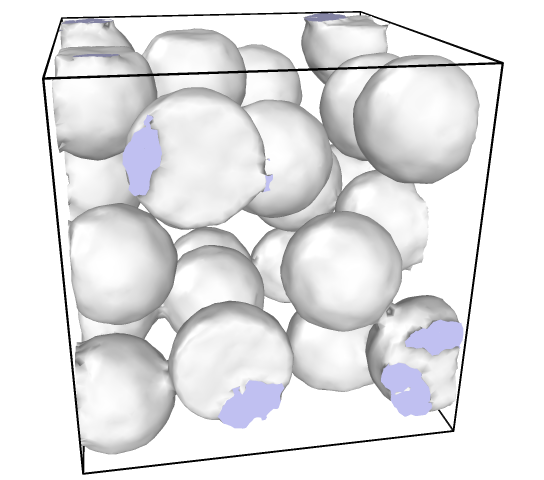
\includegraphics[width=10cm]{Cap_5/spheres2.png}
  \caption[Imágenes de la muestra]{Imágenes de la muestra.}
  \label{C5:fg:sint}
\end{figure}

\section{Automatización}
\label{AB_3}

Instrucciones de scripts acá

